\documentclass[preprint,12pt]{elsarticle}
\usepackage[T1]{fontenc}
\usepackage[utf8]{inputenc}
\usepackage[cyr]{aeguill}
\usepackage[english]{babel}
\usepackage{amsmath,amssymb,amsthm}
\usepackage{bm}
\usepackage{graphicx}

%\usepackage{natbib}
\usepackage[colorlinks=true,linkcolor=black, citecolor=blue, urlcolor=blue]{hyperref}
%\usepackage{url}

\usepackage{comment}
\usepackage{geometry}
\geometry{top=2cm,bottom=2.5cm,left=2.5cm,right=2.5cm}

\usepackage{mathrsfs}

\newcommand{\tens}[1]{%
	\mathbin{\mathop{\otimes}\displaylimits_{#1}}%
}


\DeclareMathOperator*{\argmax}{arg\,max}
\DeclareMathOperator*{\argmin}{arg\,min}
\DeclareMathOperator{\Tr}{Tr}

\usepackage{diffcoeff}

\newtheorem{theorem}{Theorem}
\newtheorem{remark}{Remark}
\newtheorem{definition}{Definition}
\newtheorem{proposition}{Proposition}

\graphicspath{{./Figures/}}

\newcommand{\matr}[1]{\bm{#1}} 

\def\onedot{$\mathsurround0pt\ldotp$}
\def\cddot{% two dots stacked vertically
	\mathbin{\vcenter{\baselineskip.67ex
			\hbox{\onedot}\hbox{\onedot}}%
}}

\makeatletter \renewcommand\d[1]{\ensuremath{%
		\;\mathrm{d}#1\@ifnextchar\d{\!}{}}}
\makeatother

%\journal{Elsevier}

\begin{document}

	\begin{frontmatter}	
		%% Title, authors and addresses
		
		%% use the tnoteref command within \title for footnotes;
		%% use the tnotetext command for theassociated footnote;
		%% use the fnref command within \author or \address for footnotes;
		%% use the fntext command for theassociated footnote;
		%% use the corref command within \author for corresponding author footnotes;
		%% use the cortext command for theassociated footnote;
		%% use the ead command for the email address,
		%% and the form \ead[url] for the home page:
		%% \title{Title\tnoteref{label1}}
		%% \tnotetext[label1]{}
		%% \author{Name\corref{cor1}\fnref{label2}}
		%% \ead{email address}
		%% \ead[url]{home page}
		%% \fntext[label2]{}
		%% \cortext[cor1]{}
		%% \address{Address\fnref{label3}}
		%% \fntext[label3]{}	
		\title{Port-Hamiltonian formulation and \\ Symplectic discretization of Plate models \\
		\vspace{2mm}\large\textit{Part I : Mindlin model for thick plates}}	
		%% use optional labels to link authors explicitly to addresses:
		%% \author[label1,label2]{}
		%% \address[label1]{}
		%% \address[label2]{}
		\author[ISAE]{Andrea Brugnoli\corref{cor1}}
		\ead{Andrea.Brugnoli@isae.fr}
		
		\author[ISAE]{Daniel Alazard}
		\ead{Daniel.Alazard@isae.fr}
		
		\author[ISAE]{Valérie Pommier-Budinger}
		\ead{Valerie.Budinger@isae.fr}
		
		\author[ISAE]{Denis Matignon}
		\ead{Denis.Matignon@isae.fr}
		
		\cortext[cor1]{Corresponding author}
		
		
		\address[ISAE]{ISAE-SUPAERO, Université de Toulouse, France.\\
		\vspace{2mm} {10 Avenue Edouard Belin, BP-54032, 31055 Toulouse Cedex 4.}}
		
		\begin{abstract}
		The port-Hamiltonian formulation is a powerful method  for modeling and interconnecting systems of different natures. In this paper, the port-Hamiltonian formulation in both vectorial and tensorial forms of a thick plate described  by the Mindlin-Reissner model is presented. Boundary control and observation are taken into account. Thanks to tensorial calculus, it can be seen that the Mindlin plate model mimics the interconnection structure of its one-dimensional counterpart, i.e. the Timoshenko beam.\\
        The Partitioned Finite Element Method (PFEM\footnote{PFEM stands for partitioned finite element method.}) is then extended to both the vectorial and tensorial formulations in order to obtain a suitable, i.e. structure-preserving, finite-dimensional port-Hamiltonian system (pHs\footnote{pHs stands for port-Hamiltonian systems.}), which preserves the structure and properties of the original distributed parameter system. Mixed boundary conditions are finally handled by introducing some algebraic constraints.
		\end{abstract}
		
		\begin{keyword}
			%% keywords here, in the form: keyword \sep keyword
			%% PACS codes here, in the form: \PACS code \sep code
			%% MSC codes here, in the form: \MSC code \sep code
			%% or \MSC[2008] code \sep code (2000 is the default)
			port-Hamiltonian systems \sep Mindlin-Reissner plate \sep Partitioned Finite Element Method \sep geometric spatial discretization \sep boundary control.		
		\end{keyword}
		
	\end{frontmatter}

	
	\section*{Introduction}
	The port-Hamiltonian (PH) formalism is acquiring more visibility for its capability to represent a huge class of systems coming from different realms of physics. A main feature of this framework is its modularity. Finite-dimensional port-Hamiltonian systems can be easily interconnected together, as shown in \cite{Cervera2007}, allowing the construction of complex multi-physics systems. The interconnection is possible also in the infinite-dimensional case \cite{ShaftIntInfinite}, even if the procedure is not as straightforward as in the finite-dimensional case. Eventually, it is also possible to merge finite and infinite PH systems \cite{vanderShaftintFinInf}. These features and capabilities are particularly appealing for control engineers in order to simplify the modeling task in preliminary analyses. \\
	
	
	Distributed parameter systems are of relevant interest given the increased computational power available for simulations. PH distributed systems were initially presented in \cite{VANDERSCHAFT2002166}, by using the theory of differential forms. Links towards functional analysis have been made in \cite{Villegas} and an exhaustive reference about the subject can be found in \cite{BookZwart}. The fundamental feature of a distributed PH system is the underlying geometric interconnection structure, the so-called Stokes-Dirac structure, that describes the power flow across the boundary and inside the system, together with an energy functional, the Hamiltonian, that determines the nature of the system. Linear/nonlinear, parabolic/hyperbolic systems can be all recast into this framework, \cite{bookPHs}. Port-Hamiltonian systems are by definition open systems, able to interact with the environment through boundary ports. The definitions of these boundary variables is of utmost importance to show that a PH system is well posed ( see \cite{LeGorrec2005} for the proof in the 1D case). Applications coming from continuum mechanics, electrodynamics and thermodynamics can be integrated inside this framework. Academic examples typically considered are the transmission line, the shallow water equations and the Maxwell equations \cite{PHbookShaft}. \\
	
	Numerical simulations and control techniques require a spatial discretization that is meant to preserve the underlying properties related to power continuity. The discretization procedure for systems under PF formalism consists of two steps:
	\begin{itemize}
		\item Finite-dimensional approximation of the Stokes-Dirac structure, i.e. the formally skew symmetric differential operator that defines the structure. The duality of the power variables has to be mapped onto the finite approximation. The subspace of the discrete variables will be represented by a Dirac structure. 
		\item The Hamiltonian requires as well a suitable discretization, which gives rise to a discrete Hamiltonian. 
	\end{itemize} 
	
	The research community is focusing on structure-preserving discretization techniques since several years. In \cite{Golo}, the authors made use of a mixed finite element spatial discretization for 1D hyperbolic system of conservation laws, introducing different low-order basis functions for the energy and co-energy variables. Pseudo-spectral methods relying on higher-order global polynomial approximations were studied in \cite{moulla:hal-01625008}. This method was used and extended to take into account unbounded control operators in \cite{confFlavio}. More recently a simplicial discretization based on discrete exterior calculus was proposed in \cite{SESLIJA20121509}. This approach comes with additional complexities, since a primal and a dual meshes have to be defined but the discretization is structure-preserving, regardless of the spatial dimension of the problem. Weak formulations which lead to Galerkin numerical approximations began to be explored in the last years. In \cite{WeakForm_Kot} the prototypical example of hyperbolic systems of two conservation law was discretized by a weak formulation. In this approach the boundary is split according to the causality of boundary ports, so that mixed boundary conditions are easily handled, but still dual meshes have to be defined.  \\
	
	The main contributions of this paper is the enrichment of the port-Hamiltonian formulation for the Mindlin plate model, by making use of tensor calculus (see \cite[Chapter~16]{Grinfield}), together with a consistent discretization method.  This kind of model was already presented in \cite{MacchelliMindlin} but here a novel formulation based on tensorial calculus is introduced. The second contribution of this paper concerns the extension of the Partitioned Finite Element Method (PFEM) to the Mindlin plate model. In this approach, originally presented in \cite{CardosoRibeiro2018}, once the system has been put into weak form, a subset of the equations is integrated by parts, so that boundary variables are naturally included into the formulation and appear as control inputs, the collocated outputs being defined accordingly. Then, the discretization of energy and co-energy variables (and the associated test functions) leads directly to a full rank representation for the finite-dimensional port-Hamiltonian system. If mixed boundary conditions are to be considered, the finite-dimensional system contain constraints, leading to an algebraic differential system (DAE), which can be treated and analyzed by referring to \cite{vanderSchaft2013, beattie2017port}. This approach, similarly to the one detailed in \cite{WeakForm_Kot}, makes possible the usage of FEM software, like FEniCS \cite{LoggMardalEtAl2012}. The final discretized system can be further reduced by using appropriate model reduction techniques, as explained in \cite{TONG20132727, Mehrmann2018}  \\
	
	The paper is divided into four main sections 
	\begin{enumerate}
		\item The framework of finite-dimensional port-Hamiltonian systems (pHs) and the notion of Dirac structure systems are recalled. The infinite-dimensional case is then illustrated by means of the Timoshenko beam model, the 1D counterpart of the Mindlin plate model.
		\item The constitutive relations and variational formulation for the Mindlin-Reissner plate is detailed. The latter arises from the Hamilton's principle and makes appear the kinetic and potential energies, that is used to define the Hamiltonian.
		\item The port-Hamiltonian formulation is highlighted by defining energy and co-energy variables and the interconnection structure. The boundary variables are found by introducing the energy balance. Then the underlying Stokes-Dirac structure is easily obtained by defining the flow and effort spaces, together with the space of boundary variables.
		\item Finally, the PFEM discretization is detailed. The problem is put into weak form first, then the necessary integrations by parts are performed and finally the basis functions for the energy, co-energy and test functions are chosen.
	\end{enumerate}


	
\section{Recall on port-Hamiltonian systems}
In this section the general nomenclature and framework for finite-dimensional and infinite-dimensional Hamiltonian system are detailed. To illustrate the infinite-dimensional case, the Timoshenko beam is considered as a first example in 1D.

\subsection{Finite-dimensional PHs}
Consider the time-invariant port-Hamiltonian system of
the form
\begin{equation}
\label{eq:finitePH}
\begin{cases}
\dot{ \bm{x} } &= (J(\bm{x}) - R(\bm{x})) \nabla H(\bm{x}) + B(\bm{x})\bm{u}, \\
\bm{y} &= B(\bm{x})^T \nabla H(\bm{x}),
\end{cases}
\end{equation}

where $\bm{x} \in \mathbb{R}^{n}$ is the state vector (also called  energy variables), $ H(\bm{x}) : \mathbb{R}^{n} \rightarrow \mathbb{R} $ is the Hamiltonian, $J \in \mathbb{R}^{n \times n}$ the skew-symmetric interconnection matrix and $R \in \mathbb{R}^{n \times n}$ the symmetric positive semi-definite dissipation or damping matrix.  Matrix $J$ represents the exchange of energy between the storage elements of the system, while dissipation is characterized by $R$. The
input matrix $B \in \mathbb{R}^{n \times m}$ and the gradient $\nabla H(\bm{x})$ of the energy function define the collocated output $\bm{y} \in \mathbb{R}^{m}$ which, together with the input $\bm{u} \in \mathbb{R}^{m}$, constitutes the power port $(\bm{u}, \bm{y})$ of the system. The power flow that goes into the system is given by
\begin{equation}
\begin{aligned}
\dot{H}(\bm{x}) &= \nabla^T{H(\bm{x})} [(J(\bm{x}) - R(\bm{x})) \nabla H(\bm{x}) + B(\bm{x})\bm{u} ], \\ 
&= - \nabla^T{H(\bm{x})} R(\bm{x}) \, \nabla{H(\bm{x})} + \bm{y}^T \bm{u}, \\
&\le \bm{y}^T \bm{u} \qquad \text{since } R(\bm{x}) \succeq 0.
\end{aligned}
\end{equation}
If $H(\bm{x})$ is positive definite, Lyapunov stability of the unforced system follows directly. However, if $H(\bm{x})$ is only
semi-definite, zero-state detectability is necessary in addition. Asymptotic stability of the port-Hamiltonian system can be checked by the invariance principle of LaSalle. In the case of stationary linear port-Hamiltonian systems, the Hamiltonian is a quadratic energy function
\begin{equation}
H(\bm{x}) =\frac{1}{2} \bm{x}^T Q \bm{x},
\end{equation}
with $Q \in \mathbb{R}^{n \times n}$ symmetric and positive definite. Furthermore, the matrices $J, R, B$ are constant matrices, independent of the state vector $\bm{x}$.  The gradient of the Hamiltonian is  linear in $\bm{x}$, and given by $\nabla H(\bm{x}) = Q \bm{x}$. In the port-Hamiltonian framework this vector goes under the name of co-energy variables and is denoted by $\bm{e}$.

It is also possible to rewrite \eqref{eq:finitePH} assuming $R = 0$ as
\begin{equation}
\label{eq:Smatrix}
\begin{pmatrix}
-\dot{ \bm{x} }\\
\bm{y} \\
\end{pmatrix} = 
\underbrace{\begin{bmatrix}
-J(\bm{x}) & -B(\bm{x}) \\
B(\bm{x})^T & 0 \\
\end{bmatrix}}_{{S}(\bm{x})}
\begin{pmatrix}
\nabla H(\bm{x})\\
\bm{u} \\
\end{pmatrix}.
\end{equation}
Note that the dynamics of the port-Hamiltonian system is provided by an interconnection structure (here given by the ${S}(\bm{x})$ matrix), together with the Hamiltonian.

\subsubsection{Dirac Structure}
Following e.g. \cite{PHbookShaft}, given the linear spaces $\mathcal{F}$ and $\mathcal{E}$, whose elements are labeled as $\bm{f}$ (flows) and $\bm{e}$ (efforts) respectively, the bond space (or power
space) is defined as: $\mathcal{B} := \mathcal{F} \times \mathcal{E}$, with elements denoted by $\bm{b} := (\bm{f}, \bm{e})$. The spaces $\mathcal{F}$ and $\mathcal{E}$ are power conjugate. This means that there exists a map $< \vert >$ defined as
\begin{equation}
\begin{aligned}
& \left\langle \; \vert \; \right\rangle :\mathcal{F} \times \mathcal{E} \rightarrow \mathbb{R}, \\
& \forall (\bm{f}, \bm{e}) \rightarrow P = \left\langle \bm{e} \vert \bm{f} \right\rangle,
\end{aligned}
\end{equation}


where $\left\langle \vert \right\rangle$ is called power product. This product should satisfy the following conditions:
\begin{itemize}
\item it is a linear function of each coordinate,
\item it is non-degenerate, that is:
\begin{itemize}
\item if $\left\langle \bm{e} \vert \bm{f} \right\rangle = 0, \; \forall \bm{e} \in \mathcal{E}$, then $\bm{f} = 0$;
\item if $\left\langle \bm{e} \vert \bm{f} \right\rangle = 0, \; \forall \bm{f} \in \mathcal{F}$, then $\bm{e} = 0$;
\end{itemize}
\item $P$ has the physical dimension of power.
\end{itemize}

$\mathcal{F}$ is called flow space, $\bm{f}$ flow variable, $\mathcal{E}$ effort space and $\bm{e}$ effort variable. 
One example of possible power product is the inner product of finite-dimensional vector spaces. Closely related to the definition of power product, there exist a symmetric bilinear form defined by
\begin{equation}
\label{eq:bil_form}
\begin{aligned}
&\ll (\bm{f}^a, \bm{e}^a), (\bm{f}^b, \bm{e}^b) \gg := \left\langle \bm{e}^a \vert \bm{f}^b  \right\rangle+ \left\langle \bm{e}^b \vert \bm{f}^a \right\rangle, \\
&(\bm{f}^a, \bm{e}^a), (\bm{f}^b, \bm{e}^b) \in \mathcal{F} \times \mathcal{E}.
\end{aligned}
\end{equation}

The relationship between the power product and the bilinear form is given by
\begin{equation}
\ll (\bm{f}, \bm{e}), (\bm{f}, \bm{e}) \gg = 2 \left\langle \bm{e} \vert \bm{f} \right\rangle.
\end{equation}

\begin{definition}[Dirac Structure]
A Dirac structure on $\mathcal{B} := \mathcal{F} \times \mathcal{E}$ is a subspace $\mathcal{D} \subset \mathcal{B}$, such that $\mathcal{D} = \mathcal{D}^\perp$, where $\perp$ denotes orthogonal complement with respect to the bilinear form $\ll , \gg$ \eqref{eq:bil_form}.
\end{definition}

Let us recall the port-Hamiltonian system presented in \eqref{eq:Smatrix}, flow variables are defined
as
\begin{align}
\bm{f} &:=
\begin{pmatrix}
-\dot{ \bm{x} }\\
\bm{y} \\
\end{pmatrix}, \quad \bm{f} \in \mathcal{F}, \\
\bm{e} &:=
\begin{pmatrix}
\nabla H(\bm{x})\\
\bm{u} \\
\end{pmatrix}, \quad \bm{e} \in \mathcal{E},
\end{align}
then a relationship between the flow and effort variables can be written as $\bm{f} = S \bm{e}$ with $S$ skew-symmetric, as it can be readily checked in \eqref{eq:Smatrix}.

\subsection{Infinite-dimensional PHs}
Following \cite{LeGorrec2005}, the prototypical example of the Timoshenko beam will be used to illustrate the class of distributed port-Hamiltonian systems. This model consists of two coupled PDEs, describing the vertical displacement and rotation scalar fields
\begin{equation}
\begin{cases}
\displaystyle \rho(x) \diffp[2]{w}{t}(x,t) &= \displaystyle \diffp{}{x} \left[K(x) \left(\diffp{w}{x}(x,t) - \phi(x,t)\right)\right], \quad x \in (0,L),\, t \ge 0 \\
\displaystyle I_{\rho}(x) \diffp[2]{\phi}{t}(x,t) &= \displaystyle \diffp{}{x} \left(EI(x) \diffp{ \phi}{x}(x,t)\right) + K(x) \left(\diffp{w}{x}(x,t) - \phi(x,t) \right),
\end{cases}
\end{equation}
where ${w}(x,t)$ is the transverse displacement and $\phi(x,t)$ is the rotation angle of a fiber of the beam. The coefficients $\rho(x), I_{\rho}(x), E(x), I(x)$ and $K(x)$ are the mass per unit length, the rotary moment of inertia of a cross section, Young's modulus of elasticity, the moment of inertia of a cross section and the shear modulus, respectively. The energy variables are chosen as follows
\begin{equation}
\begin{aligned}
\alpha_{w} &:= \rho(x) \diffp{w}{t}(x,t), \\
\alpha_{\phi} &:= I_{\rho}(x) \diffp{\phi}{t}(x,t), \\
\alpha_{\kappa} &:= \diffp{\phi}{x}(x,t), \\
\alpha_{\gamma} &:= \diffp{w}{x}(x,t) - \phi(x,t). \\
\end{aligned}
\end{equation}

Those variables are collected in the vector $\bm{\alpha} := (\alpha_{w}, \, \alpha_{\phi}, \, \alpha_{\kappa}, \, \alpha_{\gamma} )^T $, so that the Hamiltonian can be written as a quadratic functional in the energy variables 
\begin{equation}
H = \frac{1}{2} \int_{0}^{L} \bm{\alpha}^T Q \bm{\alpha} \; dx,
\qquad \text{where} \qquad
Q = 
\begin{bmatrix}
\frac{1}{\rho(x)} & 0 & 0 & 0 \\
0 & \frac{1}{I_{\rho}(x)} & 0 & 0 \\
0 & 0 & EI(x) & 0 \\
0 & 0 & 0 & K(x) \\
\end{bmatrix}.
\end{equation}

The co-energy variables are found by computing the variational derivative of the Hamiltonian (see  \cite{MacchelliTimo})
\begin{equation}
\begin{aligned}
e_{w} &:= \diffd{H}{\alpha_w} = \diffp{w}{t}(x,t), \\
e_{\phi} &:= \diffd{H}{\alpha_{\phi}} = \diffp{\phi}{t}(x,t), \\
e_{\kappa} &:= \diffd{H}{\alpha_{\kappa}} =EI(x) \diffp{\phi}{x}(x,t), \\
e_{\gamma} &:= \diffd{H}{\alpha_{\gamma}} = K(x) \left(\diffp{w}{x}(x,t) - \phi(x,t) \right). \\
\end{aligned}
\end{equation}
Those variables are again collected in the vector $\bm{e} = (e_{w}, \, e_{\phi}, \, e_{\kappa}, \, e_{\gamma} )^T $, so that the underlying interconnection structure is then found to be
\begin{equation}
\label{eq:PH_Timo}
\diffp{\bm{\alpha}}{t} = J \mathbf{e},  	\qquad \text{where} \qquad
J = 
\begin{bmatrix}
0 & 0 & 0 & \diffp{}{x} \\
0 & 0 & \diffp{}{x} & 1  \\
0 & \diffp{}{x} & 0 & 0 \\
\diffp{}{x} & -1 & 0 & 0 \\
\end{bmatrix} .
\end{equation}

For an infinite-dimensional system, boundary variables have to be defined as well. Those are found by evaluating the energy rate flow across the boundary. One possible choice among others (as illustrated in \cite{LeGorrec2005}) for this model is the following 

\begin{equation}
\bm{f}_{\partial} = 
\begin{pmatrix}
e_w(0) \\
e_{\phi}(0) \\
e_{\gamma}(L) \\
e_{\kappa}(L) \\
\end{pmatrix}, \qquad
\bm{e}_{\partial} = 
\begin{pmatrix}
-e_{\gamma}(0) \\
-e_{\kappa}(0) \\
e_{w}(L) \\
e_{\phi}(L) \\
\end{pmatrix}.
\end{equation}

The flow variables can now be defined as $\bm{f} = - \diffp{\bm{\alpha}}{t}$, so that the flow space is given by the tuples
$(\bm{f},\bm{f}_{\partial}) \in \mathcal{F}$. Equivalently the effort space is given by $(\bm{e},\bm{e}_{\partial}) \in \mathcal{E}$. The power space is therefore the Cartesian product of the two
\begin{equation}
	\mathcal{B} := \left\{(\bm{f},\bm{f}_{\partial},\bm{e},\bm{e}_{\partial}) \in \mathcal{F} \times \mathcal{E} \right\}.
\end{equation}

The duality pairing between elements of $\mathcal{B}$ is then defined as follows
\begin{equation}
\label{eq:bil_Timo}
\ll ((\bm{f}^a,\bm{f}_{\partial}^a), (\bm{e}^a,\bm{e}_{\partial}^a)), ((\bm{f}^b,\bm{f}_{\partial}^b), (\bm{e}^b,\bm{e}_{\partial}^b)) \gg := \int_{0}^{L}\left\{ (\bm{f}^{a})^T \bm{e}^b + (\bm{f}^{b})^T \bm{e}^a \right\} dx + (\bm{f}_{\partial}^{a})^T \bm{e}_{\partial}^b + (\bm{f}_{\partial}^{b}) ^T \bm{f}_{\partial}^a.
\end{equation}
The Stokes-Dirac structure of the Timoshenko beam is therefore the following
\begin{theorem}[From \cite{MacchelliTimo}, Stokes-Dirac Structure for the Timoshenko beam]
Consider the space of power variables $\mathcal{F} \times \mathcal{E}$ and the bilinear form $\ll , \gg$ given by \eqref{eq:bil_Timo}; define the following linear subspace $\mathcal{D} \subset \mathcal{F} \times \mathcal{E}$
\begin{equation}
\mathcal{D} =  \left\{(\bm{f},\bm{f}_{\partial},\bm{e},\bm{e}_{\partial}) \in \mathcal{F} \times \mathcal{E} | \; \bm{f} = -J\bm{e},  \quad
\begin{aligned}
\bm{f}_{\partial} &= 
\begin{pmatrix}
e_w(0) & e_{\phi}(0) & e_{\gamma}(L) & e_{\kappa}(L) \\
\end{pmatrix}^T \\
\bm{e}_{\partial} &= 
\begin{pmatrix}
-e_{\gamma}(0) & -e_{\kappa}(0) & e_{w}(L) & e_{\phi}(L) \\
\end{pmatrix}^T
\end{aligned} \right\}.
\end{equation}
Then $\mathcal{D} = \mathcal{D}^{\perp}$, i.e $\mathcal{D}$ is a Dirac structure.
\end{theorem}


\section{Mindlin theory for thick plates}
In this section the classical variational approach (Hamilton's principle) to derive the equations of motions is first detailed. 
\subsection{Model and associated variational formulation}
\label{sec:Min_Var}
The Mindlin plate theory, originally presented in \cite{mindlin}, is more suited for plates having a large thickness. The fibers of the plate are supposed to remain straight after the deformation, but not necessarily normal to the mid-plane. For this reason two new kinematic variables have to be added, in order to represent the deflection of the cross section along the $x$ (corresponding to angle $\psi_y$) and $y$ axis (corresponding to angle $-\psi_x$). The displacement field is therefore given by the following relations
\begin{equation}
u(x,y,z) = -z \psi_x, \qquad v(x,y,z) = -z \psi_y, \qquad 
w(x,y,z) = w(x,y).
\end{equation}
The strain field can be separated into bending and shear $\bm{\epsilon} = \left(\bm{\epsilon}_b, \; \bm{\epsilon}_s \right)^T$ with
\begin{equation}
\bm{\epsilon}_b = 
\begin{pmatrix}
\epsilon_{xx} \\
\epsilon_{yy} \\
\gamma_{xy} \\
\end{pmatrix} = -z
\begin{pmatrix}
\diffp{\psi_x}{x} \\
\diffp{\psi_y}{y} \\
\diffp{\psi_y}{x} + \diffp{\psi_x}{y} \\
\end{pmatrix} = -z
\begin{pmatrix}
\kappa_{xx} \\
\kappa_{yy} \\
\kappa_{xy} \\
\end{pmatrix} = -z \bm{\kappa}\,,
\end{equation}
and
\begin{equation}	
\bm{\epsilon}_s = 
\begin{pmatrix}
\gamma_{xz} \\
\gamma_{yz} \\
\end{pmatrix} = 
\begin{pmatrix}
\diffp{w}{x} - \psi_x \\
\diffp{w}{y} - \psi_y \\
\end{pmatrix}.
\end{equation}

For thick plates it is convenient to split the constitutive law into bending and shear contribution
\begin{equation}
\bm{\sigma} = 
\begin{pmatrix}
\bm{\sigma}_b \\
\bm{\sigma}_s \\
\end{pmatrix} = 
\begin{bmatrix}
\bm{E}_b & 0 \\
0 & \bm{E}_s \\
\end{bmatrix}
\begin{pmatrix}
\bm{\epsilon}_b \\
\bm{\epsilon}_s \\
\end{pmatrix},
\qquad
\bm{\sigma}_b = 
\begin{pmatrix}
\sigma_{xx} \\
\sigma_{yy} \\
\sigma_{xy} \\
\end{pmatrix},
\qquad
\bm{\sigma}_s = 
\begin{pmatrix}
\sigma_{xz} \\
\sigma_{yz} \\
\end{pmatrix}.
\end{equation}

The matrices $\bm{E}_b, \bm{E}_s$ for an isotropic material take the form\begin{equation}
\bm{E}_b =
\frac{E}{1 - \nu^2}
\begin{bmatrix}
1 & \nu & 0 \\
\nu & 1 & 0 \\
0  &  0 & \frac{1-\nu}{2}\\
\end{bmatrix},
\qquad
\bm{E}_s = 
\begin{bmatrix}
G & 0 \\
0 & G \\
\end{bmatrix},
\end{equation}
where $G=\frac{E}{2(1 + \nu)}$ is the shear modulus and $\nu$ is the Poisson modulus.
The stresses integrated along the thickness $h$ generate momenta and forces as follows
\begin{equation}
\begin{pmatrix}
\bm{M} \\
\bm{Q} \\
\end{pmatrix} = \int_{-\frac{h}{2} }^{\frac{h}{2}}
\begin{pmatrix}
-z \bm{\sigma}_b \\
\bm{\sigma}_s \\
\end{pmatrix} \d{z}=
\begin{bmatrix}
\bm{D}_b & 0 \\
0 & \overline{\bm{D}}_s \\
\end{bmatrix}
\begin{pmatrix}
\bm{\kappa} \\
\bm{\epsilon}_s \\
\end{pmatrix}.
\end{equation}
Matrices $\bm{D}_b$ and $\overline{\bm{D}}_s$ come from the integration along the fiber of the constitutive relation
\begin{equation}
\bm{D}_b = \int_{-\frac{h}{2} }^{\frac{h}{2}} z^2 \bm{E}_b \; \d{z}, \qquad
\overline{\bm{D}}_s = \int_{-\frac{h}{2} }^{\frac{h}{2}} \bm{E}_s \; \d{z}.
\end{equation}
Since the kinematic model of the plate is too stiff, a correction factor $k$ is introduced inside matrix $\overline{\bm{D}}_s$ and we define $\bm{D}_s$ such that $\bm{D}_s = k \overline{\bm{D}}_s$. Below the corrected version of the $\bm{D}_s$ matrix will be used.
If the mechanical properties are constant along the $z$-axis (but not necessarily in the $(x, y)$-plane), momenta $\bm{M} = \left(M_{xx}, \, M_{yy}, \, M_{xy} \right)^T$ and shear forces $\bm{Q} = \left(Q_{x}, \, Q_{y}\right)^T$ are related to the kinematic variables as follows
\begin{equation}
\begin{aligned}
M_{xx} &= D\left(\diffp{\psi_x}{x} + \nu \diffp{\psi_y}{y}\right),\\
M_{yy} &= D\left(\diffp{\psi_y}{y} + \nu \diffp{\psi_x}{x}\right),\\
M_{xy} &= D \frac{(1 - \nu)}{2} \left(\diffp{\psi_x}{x} + \diffp{\psi_y}{y}\right), \\
\end{aligned} \qquad
\begin{aligned}
Q_{x} &= k G h \left(\diffp{w}{x} - \psi_x \right), \\
Q_{y} &= k G h \left(\diffp{w}{y} - \psi_y \right). \\
\end{aligned}
\end{equation}

The following extrema problem (Hamilton's principle) can now be stated

\begin{equation} 
\{w_0, \psi_{x, 0}, \psi_{y, 0}\} = \{w, \psi_x, \psi_y \in \mathcal V; \; \left.\delta F(w,\psi_x, \psi_y) \right|_{w_0, \psi_{x, 0}, \psi_{y, 0}} = 0\}
\end{equation}
and
\begin{equation}
F(w, \psi_x, \psi_y) = \int_0^T \int_\Omega \left\{\mathcal{K} - \mathcal{U} + \mathcal{W} \right\} \d\Omega \, \d{t}.
\end{equation}

Again, many boundary terms and distributed loads may be added to this formulation. For sake of simplicity only a vertical distributed load is considered. In this model the external work $\mathcal{W}$ due to a distributed load $p$ and the kinetic and potential energy densities per unit area ($\mathcal{K}$ and $\mathcal{U}$), are respectively given by
\begin{align*}
\mathcal{W} &= pw, \\
\mathcal{K} &= \frac{1}{2} \rho \left[ h \left(\diffp{w}{t}\right)^2 +  \frac{h^3}{12}\left(\diffp{\psi_x}{t}\right)^2 + \frac{h^3}{12}\left(\diffp{\psi_y}{t}\right)^2 \right],\\
\mathcal{U} &= \frac{1}{2}\bm{\kappa}^T \bm{D}_b \bm{\kappa} + \frac{1}{2}\bm{\epsilon}_s^T \bm{D}_s \bm{\epsilon}_s.	
\end{align*} 

The total energy density is the sum of kinetic and potential energies
\begin{equation}
\mathcal{H} = \mathcal{K} + \mathcal{U}
\end{equation}
and the corresponding energies are given by the following relations
\begin{equation}
H = \int_{\Omega} \mathcal{H} \ \d\Omega, \qquad K = \int_{\Omega} \mathcal{K} \ \d\Omega, \qquad U = \int_{\Omega} \mathcal{U} \ \d\Omega.
\end{equation}
The Euler-Lagrange equations stemming form the variational principle read\begin{equation}
\begin{aligned}
\rho h \diffp[2]{w}{t} &= p + \diffp{Q_x}{x} + \diffp{Q_y}{y}, \\
\rho\frac{h^3}{12} \diffp[2]{\psi_x}{t} &= Q_x + \diffp{M_{xx}}{x} + \diffp{M_{xy}}{y}, \\
\rho\frac{h^3}{12} \diffp[2]{\psi_y}{t} &= Q_y + \diffp{M_{xy}}{x} + \diffp{M_{y}}{y}. \\
\end{aligned}
\end{equation}

Spatial derivatives of the accelerations have been neglected. In the sequel the external distributed load $p$ will not be considered. If needed, the port-Hamiltonian framework allows the introduction of distributed load and dissipative relations.

\section{PH formulation of the Mindlin plate}
In this section the vectorial, as recalled from \cite{MacchelliMindlin},  and the new tensorial formulation for the Mindlin plate are presented: first the more intuitive vectorial formulation is presented; second, the more involved, but most appropriate, tensorial approach is considered. 


\subsection{PH vectorial formulation of the Mindlin plate}
\label{sec:PH_vec_Min}
Following the developments presented in \cite{MacchelliMindlin}, the Mindlin plate model can be rewritten by making use of the port-Hamiltonian formalism. As usual, the energy variables and the formally skew-symmetric operator $J$, that defines the Stokes-Dirac structure, are the key elements of the formulation. The linear momenta and curvatures are chosen as energy variables. Additionally the shear strains are considered, leading to \begin{equation}
\bm{\alpha} := \left(\rho h v,\ \rho \frac{h^3}{12} \omega_x,\ \rho \frac{h^3}{12} \omega_y,\ \kappa_{xx},\ \kappa_{yy},\ \kappa_{xy},\ \gamma_{xz},\ \gamma_{yz} \right)^T,
\end{equation}
where $v = \diffp{w}{t},\ \omega_x = \diffp{\psi_x}{t},\ \omega_y = \diffp{\psi_y}{t}$. The Hamiltonian density is a quadratic function of the energy variables 

\begin{equation}
\label{eq:H_min}
\mathcal{H} = \frac{1}{2} \bm{\alpha}^T \begin{bmatrix}
\frac{1}{\rho h} & 0 & 0 & 0 & 0 \\
0 & \frac{12}{\rho h^3} & 0 & 0 & 0 \\
0 & 0 & \frac{12}{\rho h^3} & 0 & 0 \\
0 & 0 & 0 & \bm{D}_b & 0 \\
0 & 0 & 0 &  0 & \bm{D}_s \\
\end{bmatrix} \bm{\alpha}.
\end{equation}

The variational derivative provides as co-energy variables
\begin{equation}
\mathbf{e} := \diffd{H}{\bm{\alpha}} = (v,\ \omega_x, \ \omega_y,\ M_{xx},\ M_{yy},\ M_{xy},\ Q_x, \ Q_y)^T.
\end{equation}
The port-Hamiltonian system and the skew-adjoint operator relating energies and co-energies are found to be
\begin{equation}
\label{eq:PH_Min}
\diffp{\bm{\alpha}}{t} = J \mathbf{e}  	\quad \text{and} \quad
J := 
\begin{bmatrix}
0 & 0 & 0 & 0 & 0 & 0 & \diffp{}{x} & \diffp{}{y} \\
0 & 0 & 0 & \diffp{}{x} & 0 & \diffp{}{y} & 1 & 0 \\
0 & 0 & 0 & 0 & \diffp{}{y} & \diffp{}{x} & 0 & 1 \\
0 & \diffp{}{x} & 0 & 0 & 0 & 0 & 0 & 0\\
0 & 0 & \diffp{}{y} & 0 & 0 & 0 & 0 & 0\\
0 & \diffp{}{y} & \diffp{}{x} & 0 & 0 & 0 & 0 & 0\\
\diffp{}{x} & -1 & 0 & 0 & 0 & 0 & 0 & 0\\
\diffp{}{y} & 0 & -1 & 0 & 0 & 0 & 0 & 0\\
\end{bmatrix}.
\end{equation}

The boundary variables are found by evaluating the time derivative of the Hamiltonian
\begin{multline*}
\dot{H} = \int_\Omega\left\{v \left(\diffp{Q_x}{x} + \diffp{Q_y}{y}\right) + \omega_x \left(Q_x + \diffp{M_{xx}}{x} + \diffp{M_{yy}}{y} \right) + \omega_y \left(Q_y + \diffp{M_{xy}}{x} + \diffp{M_{yy}}{y} \right) \right. \\
\left.  + M_{xx} \diffp{\omega_x}{x} + M_{yy} \diffp{\omega_y}{y} + M_{xy} \left(\diffp{\omega_y}{x} + \diffp{\omega_x}{y} \right) + Q_x \left(\diffp{v}{x} -\omega_x \right) + Q_y \left(\diffp{v}{y} -\omega_y \right)  \right\} \d\Omega  \\
= \int_\Omega \left\{\diffp{}{x}\left(v Q_x + \omega_x M_{xx} + \omega_y M_{xy} \right) + \diffp{}{y}\left(v Q_y + \omega_x M_{xy} + \omega_y M_{yy} \right)  \right\} \d\Omega
\end{multline*}

\begin{figure}
	\centering
	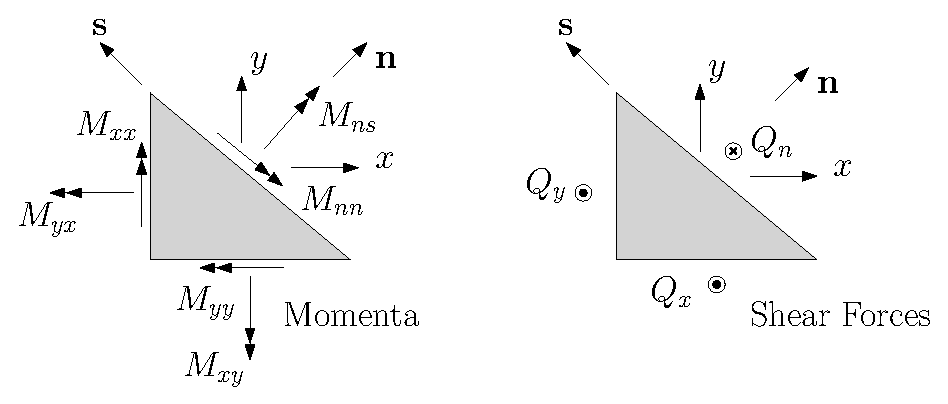
\includegraphics[width=0.7\textwidth]{Cauchy_law.eps}
	\caption{Cauchy law for momenta and forces at the boundary}
	\label{fig:Cauchy_law}
\end{figure}

	\begin{figure}[t]
	\centering
	\includegraphics[width=0.7\textwidth]{Plate_ref.eps}
	\caption{Reference frames and notations}
	\label{fig:plate_ref}
\end{figure}

Now, the following quantities, represented in Figure~\ref{fig:Cauchy_law}, are defined (see Figure~\ref{fig:plate_ref} for notations) 
\begin{equation}
\label{eq:QnMnnMns}
\begin{aligned}
\text{Shear Force} \; \; \quad Q_{n} &:= n_x Q_x + n_y Q_y   \\
\text{Flexural momentum} \quad 
M_{nn} &:= \bm{n}^T	
\begin{pmatrix}
M_{xx} n_x + M_{xy} n_y \\
M_{xy} n_x + M_{yy} n_y \\
\end{pmatrix} \\
\text{Torsional momentum} \quad M_{ns} &:= \bm{s}^T	
\begin{pmatrix}
M_{xx} n_x + M_{xy} n_y \\
M_{xy} n_x + M_{yy} n_y \\
\end{pmatrix} 
\end{aligned} \qquad
\begin{aligned}
\bm{n} &= 
\begin{pmatrix}
n_x \\
n_y \\
\end{pmatrix} \\
\bm{s} &= 
\begin{pmatrix}
-n_y \\
n_x \\
\end{pmatrix}
\end{aligned}
\end{equation}

By applying Green theorem and using definitions \eqref{eq:QnMnnMns}, together with the decomposition of the vector $(\omega_x,\ \omega_y)^T$ along the normal and tangential direction,
\begin{equation*} 
\begin{pmatrix}
\omega_x \\
\omega_y \\
\end{pmatrix}
= \begin{pmatrix}
\omega_x \\
\omega_y \\
\end{pmatrix}^T \bm{n} \,\bm{n} + \begin{pmatrix}
\omega_x \\
\omega_y \\
\end{pmatrix}^T \bm{s} \, \bm{s} = \omega_n \bm{n} +   \omega_s \bm{s},\end{equation*}
the energy balance can be expressed through the boundary values
\begin{equation}
\label{eq:energyBal_Min}
\dot{H} = \int_{\partial \Omega} \left\{v Q_n + \omega_n M_{nn} + \omega_s M_{ns}  \right\} \d{s}.
\end{equation}

This energy balance contains all the power-conjugated variables.


\subsubsection{Underlying Stokes-Dirac structure} 

This section is just a recall of what has been  presented in \cite{MacchelliMindlin} and \cite{MacchelliModelling}. Let $\mathcal{F}$ denote the flow space (for example the space of the square integrable functions on the compact set $\Omega$, i.e $L^2(\Omega, \mathbb{R}^4) \,$) and let $\mathcal{E}$ denote the effort space (for this case one possible choice is a subset of the Sobolev space $H^1(\Omega, \mathbb{R}^4)$). Equation \eqref{eq:energyBal_Min} allows identifying the boundary term of the underlying Stokes-Dirac structures. Hence the space of the boundary conditions is

\begin{equation*}
\mathcal{Z} = \{\bm{z} | \, \bm{z} = B_{\partial}(\bm{e}), \forall \, \bm{e} \in \mathcal{E} \},  \qquad \bm{z} = \left(Q_n,\ v,\ M_{nn},\ \omega_n,\ M_{ns},\ \omega_s \right)^T.
\end{equation*}

Since the formally skew-symmetric operator $J$ is a differential operator of order one, the boundary operator $B_{\partial}$ is a linear operator of order zero on the effort space. It reads

\begin{equation}
B_{\partial} = 
\begin{bmatrix}
0 & 0 & 0 & 0 & 0 & 0 & n_x & n_y \\
1 & 0 & 0 & 0 & 0 & 0 & 0 & 0\\
0 & 0 & 0 & n_x^2 & n_y^2 & 2 n_x n_y & 0 & 0 \\
0 & n_x & n_y & 0 & 0 & 0 & 0 & 0 \\ 
0 & 0 & 0 & -n_x n_y & n_x n_y & n_x^2 - n_y^2 & 0 & 0 \\
0 & -n_y & n_x & 0 & 0 & 0 & 0 & 0 \\ 
\end{bmatrix},
\end{equation}
where $n_x, n_y$ were defined in \eqref{eq:QnMnnMns}. If instead the differential operator is  of order two (like in \cite{BrugnoliKir}), the boundary operator is  a differential operator of order one on the effort space.


\begin{theorem}[From \cite{MacchelliMindlin}, Stokes-Dirac structure for the Mindlin Plate]
	The set
	\begin{equation}
	\mathcal{D} := \left\{ (\bm{f},\bm{e},\bm{z}) \in \mathcal{F}\times\mathcal{E}\times\mathcal{Z} \; | \; \bm{f}= - \diffp{\bm{\alpha}}{t} = -J \bm{e}, \; \bm{z} = B_{\partial}(\bm{e}) \right\}
	\end{equation} 
	is a Stokes-Dirac structure with respect to the pairing
	\begin{equation}
	\ll (\bm{f}_1, \bm{e}_1, \bm{z}_1), (\bm{f}_2, \bm{e}_2, \bm{z}_2) \gg  \,= \int_{\Omega} \left[ \bm{e}_1^T \bm{f}_2 + \bm{e}_2^T \bm{f}_1 \right] \d\Omega  + \int_{\partial \Omega} B_J(\bm{z}_1, \bm{z}_2) \d{s},
	\end{equation}
	where $B_J$ is a symmetric matrix  arising from the application of the Green theorem
	\begin{equation}
	\begin{aligned}
	B_J(\bm{z}_1,\bm{z}_2) 
	= \, &Q_{n,2} \ v_1 + M_{nn, 2} \ \omega_{n, 1} + M_{ns, 2} \ \omega_{s, 1} \\
	+ \, &Q_{n,1} \ v_2 + M_{nn, 1} \ \omega_{n, 2} + M_{ns, 1} \ \omega_{s, 2} \\
	= &\bm{z}_1^T \, B_J \, \bm{z}_2 \\
	\end{aligned} \, ,  \qquad
  	B_J = 
	\begin{bmatrix}
	0 & 1 & 0 & 0 & 0 & 0 \\
	1 & 0 & 0 & 0 & 0 & 0 \\
	0 & 0 & 0 & 1 & 0 & 0 \\
	0 & 0 & 1 & 0 & 0 & 0 \\ 
	0 & 0 & 0 & 0 & 0 & 1 \\
	0 & 0 & 0 & 0 & 1 & 0 \\ 
	\end{bmatrix}.
	\end{equation}
\end{theorem}



\subsection{PH tensorial formulation of the Mindlin plate}
\label{sec:PH_ten_Min}

A vectorial notation was first used for the curvatures and momenta. These variables are of intrinsically tensorial nature and in the following, the tensorial formulation takes the place of the vectorial one. First let us rewrite the momenta and curvatures as symmetric matrices (corresponding to the choice of a Cartesian frame for the representation of tensors)

\begin{equation}
\mathbb{K} = 
\begin{bmatrix}
\kappa_{xx} &  \kappa_{xy}\\
\kappa_{xy} & \kappa_{yy} \\
\end{bmatrix}, \qquad
\mathbb{M}=
\begin{bmatrix}
M_{xx} & M_{xy} \\
M_{xy} & M_{yy} \\
\end{bmatrix},
\end{equation}
where now, with a slight abuse of notation,  $\kappa_{xy}$ now is half the value of the one in the vectorial case, i.e. $\kappa_{xy} =\frac{1}{2}\left(\diffp{\psi_y}{x} + \diffp{\psi_x}{y} \right)$. All the other quantities stay the same as explained in section~\ref{sec:Min_Var}. The curvatures tensor is the linear deformation tensor applied to the rotation vector $\bm{\theta} = (\psi_x, \psi_y)^T$
\begin{equation}
\mathbb{K} = \mathrm{Grad}(\bm{\theta}) =  \frac{1}{2} \left(\nabla \tens{} \bm{\theta} + \left(\nabla \tens{} \bm{\theta}\right)^T \right).
\end{equation}
The tensor $\mathrm{Grad}(\bm{\theta})$ stands for the symmetric gradient of the vector $\bm{\theta}$.
This highlights the fact that, in the Mindlin model, rotations $\psi_x, \psi_y$ have to be treated as a vector. The Hamiltonian energy is now rewritten as
\begin{equation}
H = \int_{\Omega} \frac{1}{2} \left\{ \mu \left(\diffp{w}{t} \right)^2 +  \diffp{\bm{\theta}}{t}^T I_{\theta}  \diffp{\bm{\theta}}{t} +   \mathbb{M} \cddot \mathbb{K} + \bm{Q} \cdot \bm{\epsilon}_s  \right\}  \d\Omega, 
\end{equation}
where 
\begin{equation*}
I_{\theta} = 
\begin{bmatrix}
\frac{\rho h^3}{12} & 0 \\
0 & \frac{\rho h^3}{12} \\
\end{bmatrix}, \qquad
\begin{aligned}
\rho &= \text{Mass density}, \\
h &= \text{Thickness},
\end{aligned} 
\end{equation*}
where the tensor contraction in Cartesian coordinates is expressed as
\[\mathbb{M} \cddot \mathbb{K} = \sum_{i,j = 1}^{2} M_{ij} \kappa_{ij} = \Tr(\mathbb{M}^T \mathbb{K}).  \]
For what concerns the choice of the energy variables scalar, vector and tensor variables are grouped together
\begin{equation}
\begin{aligned}
\alpha_w &= \mu \diffp{w}{t}, \\
\mathbb{A}_{\kappa} &= \mathbb{K}, \\
\end{aligned} \qquad
\begin{aligned}
\bm\alpha_{\theta} &= I_{\theta}  \diffp{\bm{\theta}}{t}, \\
\bm\alpha_{\epsilon_s} &= \bm{\epsilon}_s. \\
\end{aligned}
\end{equation}
The co-energy variables are found by computing the variational derivative of the Hamiltonian
\begin{equation}
\begin{aligned}
e_w &:= \diffd{H}{\alpha_w} = \diffp{w}{t} := v,  \\
\mathbb{E}_{\kappa} &:= \diffd{H}{\mathbb{A}_{\kappa}} = \mathbb{M}, \\
\end{aligned} \qquad
\begin{aligned}
\bm{e}_{\theta} &:= \diffd{H}{\bm\alpha_{\theta}} = \diffp{\bm{\theta}}{t}, \\
\bm{e}_{\epsilon_s} &:= \diffd{H}{\bm{\epsilon}_s} = \bm{Q}. \\
\end{aligned}
\end{equation}
\begin{proposition}
	The variational derivative of the Hamiltonian with respect to the curvatures tensor is the momenta tensor $\diffd{H}{\mathbb{A}_{\kappa}} = \mathbb{M}$.
	\begin{proof}
		The contribution due to the bending part in Hamiltonian is given by 
		\[H_b(\mathbb{K}) = \frac{1}{2} \int_{\Omega}  \mathbb{M} \cddot \mathbb{K} \; \d\Omega = \frac{1}{2} \int_{\Omega} \Tr(\mathbb{M}^T \mathbb{K}) \; \d\Omega, \]
		where the momenta tensor depends on the curvatures tensor $\mathbb{M}_{ij} = \mathbb{D}_{ijkl}\mathbb{K}_{kl} $ where $\mathbb{D} = \mathbb{D}^T$ is a fourth order symmetric positive definite tensor.
		So a variation $\delta\mathbb{K}$ of the curvatures tensor with respect to a given value $\mathbb{K}_0$ leads to
		\[H_b(\mathbb{K}_0+ \varepsilon \delta\mathbb{K}) = \frac{1}{2} \int_{\Omega} \Tr(\mathbb{M}_0^T \mathbb{K}_0) \; \d\Omega + \varepsilon \frac{1}{2} \int_{\Omega} \left\{ \Tr(\mathbb{M}_0^T \delta\mathbb{K}) + \Tr(\delta\mathbb{M}^T \mathbb{K}_0)\right\}\; \d\Omega  + O(\varepsilon^2). \]
		The term $\Tr(\delta\mathbb{M}^T \mathbb{K}_0)$ can be further manipulated as follows 
		\[ \Tr(\delta\mathbb{M}^T \mathbb{K}_0) = \Tr(\mathbb{K}_0^T \delta\mathbb{M}) = \Tr(\mathbb{K}_0^T \, \mathbb{D} \, \delta\mathbb{K}) = \Tr(\mathbb{M}_0^T \delta\mathbb{K}),
		\]
		 so that 
		\[H_b(\mathbb{K}_0+ \varepsilon \delta\mathbb{K}) = \frac{1}{2} \int_{\Omega} \Tr(\mathbb{M}_0^T \mathbb{K}_0) \; \d\Omega + \varepsilon \int_{\Omega} \left\{ \Tr(\mathbb{M}_0^T \delta\mathbb{K})\right\}\; \d\Omega  + O(\varepsilon^2). \]
		By definition of the variational derivative (see e.g. \cite{VANDERSCHAFT2002166}) it can be written
		\[H_b(\mathbb{K}_0+ \varepsilon \delta\mathbb{K}) = H_b(\mathbb{K}_0) + \varepsilon \left\langle \diffd{H_b}{\mathbb{K}} , \delta\mathbb{K}  \right\rangle_{\mathscr{H}} + O(\varepsilon^2), \]
		where $\mathscr{H}$ is the space of the square integrable symmetric tensors endowed with the integral of the tensor contraction as inner product. By identification then $\diffd{H_b}{\mathbb{K}} = \diffd{H}{\mathbb{K}} = \mathbb{M}_0$.
	\end{proof}
\end{proposition}


Let us denote $\mathrm{div}()$ and $\mathrm{Div}()$ the divergence of a vector and of a tensor, respectively:
\begin{equation*}
    \bm{\varepsilon} = \mathrm{Div}(\mathbb{E})  \qquad \text{with } \bm{\varepsilon}_i = \mathrm{div}(\mathbb{E}_{ji}) = \sum_{j = 1}^n \diffp{\mathbb{E}_{ji}}{x_j}.
\end{equation*}
The port-Hamiltonian system is expressed as follows 
\begin{equation}
\begin{cases}
\displaystyle\diffp{\alpha_w}{t} &= \mathrm{div}(\bm{e}_{\epsilon_s}), \vspace{1mm} \\
\displaystyle\diffp{\bm\alpha_\theta}{t} &= \mathrm{Div}( \mathbb{E}_{\kappa}) + \bm{e}_{\epsilon_s}, \vspace{1mm} \\
\displaystyle\diffp{\mathbb{A}_\kappa}{t} &= \mathrm{Grad}(\bm{e}_{\theta}), \vspace{1mm} \\
\displaystyle\diffp{ \bm\alpha_{\epsilon_s} }{t} &= \mathrm{grad}(e_w) - \bm{e}_{\theta},
\end{cases}
\end{equation}

If the variables are concatenated together, the formally skew-symmetric operator $J$ can be highlighted 
\begin{equation}
\label{eq:PH_sys_Min_Ten}
\diffp{}{t}
\begin{pmatrix}
\alpha_w \\
\bm\alpha_\theta \\
\mathbb{A}_\kappa \\
\bm\alpha_{\epsilon_s} \\
\end{pmatrix} = 
\underbrace{\begin{bmatrix}
	0  & 0  & 0  & \mathrm{div} \\
	0 & 0 &  \mathrm{Div} & \bm{I}_{2 \times 2}\\
	0  & \mathrm{Grad}  & 0  & 0\\
	\mathrm{grad} & -\bm{I}_{2 \times 2} &  0 & 0  \\
	\end{bmatrix}}_{J}
\begin{pmatrix}
e_w \\
\bm{e}_{\theta} \\
\mathbb{E}_{\kappa} \\
\bm{e}_{\epsilon_s} \\
\end{pmatrix},
\end{equation}
where all zeros are intended as nullifying operators from the space of input variables to the space of output variables.
\begin{remark}
It can be observed that the interconnection structure given by $J$ in \eqref{eq:PH_sys_Min_Ten} mimics that of the Timoshenko beam given in \eqref{eq:PH_Timo}. This is not obvious if system \eqref{eq:PH_Min} is considered.
\end{remark}


\begin{theorem}{The adjoint of the tensor divergence $\mathrm{Div}$ is $- \mathrm{Grad}$, the opposite of the symmetric gradient.}
	\begin{proof}
	Let us consider the Hilbert space of the square integrable symmetric tensors of size $n \times n$ over an open connected set $\Omega$. This space will be denoted by $\mathscr{H}_1 = [L^2_{\text{sym}}(\Omega)]^{n \times n}$. This space is endowed with the integral of the tensor contraction as scalar product
	\[\left\langle \mathbb{E} , \mathbb{F} \right\rangle_{\mathscr{H}_1} = \int_{\Omega}  \mathbb{E} \cddot \mathbb{F} \; \d\Omega = \int_{\Omega} \Tr(\mathbb{E}^T \mathbb{F}) \; \d\Omega, \quad \forall \mathbb{E} , \mathbb{F} \in [L^2_{\text{sym}}(\Omega)]^{n \times n}. \]
	
	 Moreover the Hilbert space of the square integrable vector functions over the same open connected set $\Omega$ will be denoted by $\mathscr{H}_2 = [L^2(\Omega)]^n$. This space is endowed with the following scalar product
	 \[\left\langle \bm{\varepsilon} , \bm{\phi} \right\rangle_{\mathscr{H}_2} = \int_{\Omega}  \bm{\varepsilon} \cdot \bm{\phi} \; \d\Omega = \int_{\Omega} \bm{\varepsilon}^T \bm{\phi}\; \d\Omega, \quad \forall \bm{\varepsilon}, \bm{\phi} \in [L^2(\Omega)]^{n}. \]
	 Let us consider the tensor divergence operator defined as 
	 \[
	 \begin{aligned}
	 A: \; \mathscr{H}_1& \rightarrow \mathscr{H}_2, \\
	 \mathbb{E}& \rightarrow \mathrm{Div}(\mathbb{E}) = \bm{\varepsilon}, \\
	 \end{aligned}
	 \qquad \text{with } \bm{\varepsilon}_i = \mathrm{div}(\mathbb{E}_{ji}) = \sum_{j = 1}^n \diffp{\mathbb{E}_{ji}}{x_j}.
	 \]
	 We try to identify $A^*$
	 \[
	 \begin{aligned}
	 A^*: \; \mathscr{H}_2& \rightarrow \mathscr{H}_1, \\
	 \bm{\phi}& \rightarrow  A^* \bm{\phi} = \mathbb{F}, \\
	 \end{aligned}
	 \]
	 such that \[
	 	 \left\langle A \mathbb{E} , \bm{\phi} \right\rangle_{\mathscr{H}_2} = \left\langle \mathbb{E} , A^* \bm{\phi} \right\rangle_{\mathscr{H}_1},
	 \begin{aligned} \qquad
	 &\forall \mathbb{E} \in \mathrm{Domain}(A) \subset \mathscr{H}_1 \\
	 &\forall \bm{\phi} \in \mathrm{Domain}(A^*) \subset \mathscr{H}_2
	 \end{aligned}
	 \]
	 Now let us take $\mathbb{E} \in [\mathcal{C}_0^1(\Omega)]^{n \times n} \subset \mathrm{Domain}(A)$ the space of differentiable symmetric tensors with compact support in~$\Omega$. Additionally $\bm{\phi}$ will belong to $\mathcal{C}_{0}^1(\Omega)^{n} \subset \mathrm{Domain}(A^*)$, the space of differentiable vector functions with compact support in~$\Omega$. Then
	 \[
	 \begin{aligned}
	 \left\langle \mathrm{Div}\mathbb{E} , \bm{\phi} \right\rangle_{\mathscr{H}_2} &= \int_{\Omega}  \bm{\varepsilon} \cdot \bm{\phi} \; \d\Omega\, \\
	 &= \int_{\Omega} \sum_{i=1}^n \sum_{j=1}^n \diffp{\mathbb{E}_{ji}}{x_j} \phi_i \; \d\Omega\,,  \\ 
	 &= - \int_{\Omega} \sum_{i=1}^n \sum_{j=1}^n \mathbb{E}_{ji} \diffp{\phi_i}{x_j} \; \d\Omega\,, \qquad \text{since the functions vanish at the boundary,}\\
	 &= - \int_{\Omega} \sum_{i=1}^n \sum_{j=1}^n \mathbb{E}_{ji} \mathbb{F}_{ji} \;\d\Omega\,,  \qquad \text{if we first chose} \quad \mathbb{F}_{ji} = \diffp{\phi_i}{x_j}\,.\\
	 \end{aligned}	 
	 \]
	 But in this latter case, it could not indeed  be stated that $\mathbb{F} \in [L^2_{\text{sym}}(\Omega)]^{n \times n}$. Now, since  $\mathbb{E} \in [L^2_{\text{sym}}(\Omega)]^{n \times n}$, $\mathbb{E}_{ji}=\mathbb{E}_{ij}$,  thus we are  allowed to further decompose the last equality as
	  
	 \[ \sum_{i,j}\mathbb{E}_{ji} \diffp{\phi_i}{x_j} = \sum_{i,j}\mathbb{E}_{ji} \frac{1}{2} \left(\diffp{\phi_i}{x_j} + \diffp{\phi_j}{x_i}  \right) = 	\sum_{i,j} \mathbb{E}_{ji} \mathbb{F}_{ji}, \qquad \text{with } \mathbb{F}_{ji}:= \frac{1}{2} \left(\diffp{\phi_i}{x_j} + \diffp{\phi_j}{x_i}  \right).
	 \]
	 Thus $\mathbb{F} \in [L^2_{\text{sym}}(\Omega)]^{n \times n}$ and it can be stated that
	 \[ \left\langle \mathrm{Div}\mathbb{E} , \bm{\phi} \right\rangle_{\mathscr{H}_2} = - \int_{\Omega} \sum_{i,j} \mathbb{E}_{ji} \frac{1}{2} \left(\diffp{\phi_i}{x_j} + \diffp{\phi_j}{x_i}  \right) \;\d\Omega = - \int_{\Omega} \sum_{i,j} \mathbb{E}_{ji} \mathbb{F}_{ji} \;\d\Omega = \left\langle \mathbb{E} , -\mathrm{Grad} \bm{\phi} \right\rangle_{\mathscr{H}_1}. \]
	 It can be concluded that the formal adjoint of $\mathrm{Div}$ is $\mathrm{Div}^* = -\mathrm{Grad}$.
	\end{proof}
\end{theorem}

Again the boundary values can be found by evaluating the time derivative of the Hamiltonian
\begin{equation}
\begin{aligned}
\dot{H}&= \int_{\Omega} \left\{ \diffp{\alpha_w}{t} e_w  + \diffp{\bm\alpha_\theta}{t} \cdot \bm{e}_\theta + \diffp{\mathbb{A}_{\kappa}}{t} \cddot \mathbb{E}_{\kappa}  + \diffp{\bm\alpha_{\epsilon_s}}{t} \cdot \bm{e}_{\epsilon_s} \right\} \d\Omega \\
&= \int_{\Omega} \left\{ \mathrm{div}(\bm{e}_{\epsilon_s}) e_w  + \left[\mathrm{Div}(\mathbb{E}_{\kappa}) + \bm{e}_{\epsilon_s} \right] \cdot \bm{e}_\theta + \mathrm{Grad}(\bm{e}_{\theta}) \cddot \mathbb{E}_{\kappa}  + (\mathrm{grad} (e_w) - \bm{e}_{\theta}) \cdot \bm{e}_{\epsilon_s} \right\} \d\Omega \\
&= \int_{\partial \Omega} \left\{ \underbrace{(\bm{n} \cdot \bm{e}_{\epsilon_s})}_{Q_n} e_w  + (\bm{n} \cdot \mathbb{E}_{\kappa}) \cdot \bm{e}_\theta \right\} \d\Omega\,, \\
&= \int_{\partial \Omega} \left\{ Q_n e_w  + (\bm{n} \cdot \mathbb{E}_{\kappa}) \cdot (\omega_n \bm{n} + \omega_s \bm{s}) \right\} \d\Omega\,, \\&= \int_{\partial \Omega} \left\{ Q_n e_w  + \omega_n  \underbrace{\bm{n}^T \mathbb{E}_{\kappa} \bm{n}}_{M_{nn}} + \omega_s \underbrace{\bm{s}^T \mathbb{E}_{\kappa} \bm{n}}_{M_{ns}} \right\} \d\Omega\,, \\
&= \int_{\partial \Omega} \left\{ Q_n e_w  + \omega_n M_{nn} + \omega_s M_{ns} \right\} \d\Omega\,.  \\
\end{aligned}
\end{equation}
\begin{remark}
Obviously this result is equivalent to the one found in the vectorial case, but the tensorial formulation is more suitable from the point of view of functional analysis since it makes appear intrinsic operators ($\mathrm{div}, \mathrm{Div}, \mathrm{grad}, \mathrm{Grad}$), regardless of the coordinate frame of choice.
\end{remark}

\section{Discretization of the Mindlin plate using a Partioned Finite Element Method (PFEM) (\cite{CardosoRibeiro2018})}
The Partioned Finite Element Method (PFEM) consists of putting the system into weak form first and of applying the integration by parts on a subset of the overall system second. For the Mindlin plate the integration by parts can be applied to first three lines of system \eqref{eq:PH_Min} and to the first two lines of system \eqref{eq:PH_sys_Min_Ten}. This choice will make appear the momenta and forces at the boundary as control inputs. Alternatively, the last five lines of system \eqref{eq:PH_Min} (or the last two of \eqref{eq:PH_sys_Min_Ten}) could have been selected to perform the integration by parts. In this latter case the linear and angular velocities at the boundary would appear as control inputs. Keeping this in mind, the most suitable choice will depend on the physical problem under consideration (leading either to \eqref{eq:WF_Min_Dyn} or to \eqref{eq:WF_Min_Kin}). 

\subsection{Weak Form for the vectorial formulation}

First both sides of system \eqref{eq:PH_Min} are multiplied by scalar test functions $v_i$ and integrated over the domain

\begin{align}
\int_{\Omega} v_1 \diffp{\alpha_1}{t} \d\Omega &= \int_{\Omega} v_1 \left(\diffp{e_7}{x} + \diffp{e_8}{y} \right) \d\Omega  \label{eq:line1_min}\\\int_{\Omega} v_2 \diffp{\alpha_2}{t} \d\Omega &= \int_{\Omega} v_2 \left(\diffp{e_4}{x} + \diffp{e_6}{y} + e_7 \right) \d\Omega  \label{eq:line2_min} \\
\int_{\Omega} v_3 \diffp{\alpha_3}{t} \d\Omega &= \int_{\Omega} v_3 \left(\diffp{e_5}{y} + \diffp{e_6}{x} + e_8 \right) \d\Omega  \label{eq:line3_min}\\
\int_{\Omega} v_4 \diffp{\alpha_4}{t} \d\Omega &= \int_{\Omega} v_4 \diffp{e_2}{x} \d\Omega   \label{eq:line4_min}\\
\int_{\Omega} v_5 \diffp{\alpha_5}{t} \d\Omega &=  \int_{\Omega} v_5 \diffp{e_3}{y} \d\Omega \\
\int_{\Omega} v_6 \diffp{\alpha_6}{t} \d\Omega &= \int_{\Omega} v_6 \left(\diffp{e_2}{y} + \diffp{e_3}{x}\right) \d\Omega\\
\int_{\Omega} v_7 \diffp{\alpha_7}{t} \d\Omega &= \int_{\Omega} v_7 \left(\diffp{e_1}{x} - e_2 \right) \d\Omega\\
\int_{\Omega} v_8 \diffp{\alpha_8}{t} \d\Omega &= \int_{\Omega} v_8 \left(\diffp{e_1}{y} - e_3 \right) \d\Omega.   \label{eq:line8_min}
\end{align}

Equation \eqref{eq:line1_min} is integrated by parts
\begin{equation}
\label{eq:line1_min_bp}
\int_{\Omega} v_1 \diffp{\alpha_1}{t} \d\Omega = -\int_{\Omega} \left\{ \diffp{v_1}{x} e_7 + \diffp{v_1}{y} e_8 \right\} \d\Omega + \int_{\partial \Omega} v_1 \underbrace{\left( e_7 n_x + e_8 n_y \right)}_{Q_n = u_{\partial, 1} } \d{s}.
\end{equation}
Equation \eqref{eq:line1_min_bp} makes naturally appear the shear forces at the boundary. For equations \eqref{eq:line2_min} and \eqref{eq:line3_min} it is obtained
\begin{equation}
\int_{\Omega} v_2 \diffp{\alpha_2}{t} \d\Omega = \int_{\Omega} \left\{ v_2 e_7 - \diffp{v_2}{x} e_4 - \diffp{v_2}{y} e_6 \right\} \d\Omega + \int_{\partial \Omega} v_2 \left( e_4 n_x + e_6 n_y \right) \d{s},
\end{equation}
\begin{equation}
\int_{\Omega} v_3 \diffp{\alpha_3}{t} \d\Omega = \int_{\Omega} \left\{ v_3 e_8 - \diffp{v_3}{y} e_5 - \diffp{v_3}{x} e_6 \right\} \d\Omega + \int_{\partial \Omega} v_3 \left( e_6 n_x + e_5 n_y \right) \d{s}.
\end{equation}
In order to get the boundary momenta, a transformation going from normal and tangential coordinates to the Cartesian ones is needed
\begin{equation}
\begin{pmatrix}
e_4 n_x + e_6 n_y \\
e_6 n_x + e_5 n_y \\
\end{pmatrix} =
\begin{pmatrix}
M_{xx} n_x + M_{xy} n_y \\
M_{xy} n_x + M_{yy} n_y \\
\end{pmatrix} =
\begin{bmatrix}
n_x & -n_y \\
n_y &  n_x \\
\end{bmatrix}
\begin{pmatrix}
M_{nn} \\
M_{ns} \\
\end{pmatrix}.
\end{equation}

Using this transformation, the boundary terms are included in the weak formulation
\begin{equation}
\label{eq:line2_min_bp}
\int_{\Omega} v_2 \diffp{\alpha_2}{t} \d\Omega = \int_{\Omega} \left\{ v_2 e_7 - \diffp{v_2}{x} e_4 - \diffp{v_2}{y} e_6 \right\} \d\Omega + \int_{\partial \Omega} v_2 n_x \underbrace{M_{nn}}_{u_{\partial, 2}}  \d{s} - \int_{\partial \Omega} v_2 n_y \underbrace{M_{ns}}_{u_{\partial, 3}} \d{s},
\end{equation}
\begin{equation}
\label{eq:line3_min_bp}
\int_{\Omega} v_3 \diffp{\alpha_3}{t} \d\Omega = \int_{\Omega} \left\{ v_3 e_8 - \diffp{v_3}{y} e_5 - \diffp{v_3}{x} e_6 \right\} \d\Omega + \int_{\partial \Omega} v_3 n_y \underbrace{M_{nn}}_{u_{\partial, 2}}  \d{s} + \int_{\partial \Omega} v_2 n_x \underbrace{M_{ns}}_{u_{\partial, 3}} \d{s}.
\end{equation}

Again, such a formulation introduces as inputs the forces and momenta at the boundary, so that the free case can be easily handled by setting $u_{\partial, 1}=0, \ u_{\partial, 2}=0, \ u_{\partial, 3}=0$.

\subsection{Weak form for the tensorial formulation}
The same procedure detailed above is now applied on system \eqref{eq:PH_sys_Min_Ten}, but in this case the test functions are of scalar, vectorial and tensorial nature. Keeping the same notation as in section \ref{sec:PH_ten_Min}, the scalar test function is denoted by $v_w$, the vectorial one by $\bm{v}_{\theta}$, $\bm{v}_{\epsilon_s}$  the tensorial one by $\mathbb{V}_{\kappa}$.

Moreover,  we choose to derive here two different boundary control configurations, which prove useful in practice: either the forces and momenta, or the kinematic variables are chosen as boundary controls.

\subsubsection{Boundary control through forces and momenta}
The first line of \eqref{eq:PH_sys_Min_Ten} is multiplied  by $v_w$ (multiplication by a scalar), the second line and the fourth by $\bm{v}_{\theta}$, $\bm{v}_{\epsilon_s}$ (scalar product of $\mathbb{R}^2$) and the third one by $\mathbb{V}_{\kappa}$ (tensor contraction).
\begin{align}
\int_{\Omega} v_w \diffp{\alpha_w}{t}  \d\Omega &=  \int_{\Omega} v_w \mathrm{div}(\bm{e}_{\epsilon_s}) \, \d\Omega,  \label{eq:wf1_min_ten}\\
\int_{\Omega} \bm{v}_{\theta} \cdot \diffp{\bm\alpha_{\theta}}{t}   \d\Omega &= \int_{\Omega} \bm{v}_{\theta} \cdot (\mathrm{Div}( \mathbb{E}_{\kappa}) + \bm{e}_{\epsilon_s}) \,  \d\Omega,  \label{eq:wf2_min_ten} \\
\int_{\Omega} \mathbb{V}_{\kappa} \cddot \diffp{\mathbb{A}_{\kappa}}{t}   \d\Omega &= \int_{\Omega} \mathbb{V}_{\kappa} \cddot \mathrm{Grad}(\bm{e}_\theta) \, \d\Omega, \label{eq:wf3_min_ten} \\
\int_{\Omega} \bm{v}_{\epsilon_s} \cdot \diffp{\bm\alpha_{\epsilon_s}}{t}   \d\Omega &= \int_{\Omega} \bm{v}_{\epsilon_s} \cdot (\mathrm{grad}({e}_{w}) - \bm{e}_{\theta}) \, \d\Omega.  \label{eq:wf4_min_ten}
\end{align}

The right-hand side of equation \eqref{eq:wf1_min_ten} has to be integrated by parts
\begin{equation}
\label{eq:line1_ten_min}
\int_{\Omega} v_w \mathrm{div}(\bm{e}_{\epsilon_s})  \d\Omega = \int_{\partial \Omega} v_w \underbrace{\bm{n} \cdot \bm{e}_{\epsilon_s}}_{Q_n}  \d{s} - \int_{\Omega} \mathrm{grad}(v_w)  \cdot \bm{e}_{\epsilon_s}  \d\Omega,\end{equation}
as well as the right-hand side of equation \eqref{eq:wf2_min_ten}
\begin{equation}
\label{eq:line2_ten_min}
\int_{\Omega} \bm{v}_{\theta} \cdot (\mathrm{Div}(\mathbb{E}_{\kappa}) + \bm{e}_{\epsilon_s})  \d\Omega = \int_{\partial \Omega} \bm{v}_{\theta} \cdot (\bm{n} \cdot \mathbb{E}_{\kappa})  \d{s} -\int_{\Omega} \left\{ \mathrm{Grad}(\bm{v}_{\theta}) \cddot \mathbb{E}_{\kappa} - \bm{v}_{\theta} \cdot \bm{e}_{\epsilon_s}\right\}  \d\Omega.
\end{equation}

The usual additional manipulation is performed on the boundary term containing the momenta, so that the proper boundary values arise
\begin{equation}
\label{eq:line1_ipbc_ten_min}
\begin{aligned}
\int_{\partial \Omega} \bm{v}_{\theta} \cdot (\bm{n} \cdot \mathbb{E}_{\kappa})  \d{s} &= \int_{\partial \Omega} \left\{\underbrace{(\bm{v}_{\theta} \cdot \bm{n})}_{v_{\omega_n}} \bm{n} + \underbrace{(\bm{v}_{\theta} \cdot \bm{s})}_{v_{\omega_s}} \bm{s} \right\} \cdot (\bm{n} \cdot \mathbb{E}_{\kappa}) \,  \d{s} \\
&= \int_{\partial \Omega} \left\{ v_{\omega_n} M_{nn} + v_{\omega_s} M_{ns} \right\}  \d{s}.
\end{aligned}
\end{equation}
So the final weak form obtained from system \eqref{eq:PH_sys_Min_Ten} reads
\begin{equation}
\label{eq:WF_Min_Dyn}
\begin{cases}
\displaystyle\int_{\Omega} v_w \diffp{\alpha_w}{t}  \d\Omega  &= - \displaystyle\int_{\Omega} \mathrm{grad}(v_w)  \cdot \bm{e}_{\epsilon_s}  \d\Omega +  \displaystyle\int_{\partial \Omega} v_w Q_n  \d{s} \vspace{2mm}\\
\displaystyle\int_{\Omega} \bm{v}_{\theta} \cdot \diffp{\bm\alpha_{\theta}}{t}   \d\Omega &=  -\displaystyle\int_{\Omega} \left\{ \mathrm{Grad}(\bm{v}_{\theta}) \cddot \mathbb{E}_{\kappa} - \bm{v}_{\theta} \cdot \bm{e}_{\epsilon_s}\right\}  \d\Omega + \displaystyle\int_{\partial \Omega} \left\{ v_{\omega_n} M_{nn} + v_{\omega_s} M_{ns} \right\}  \d{s} \vspace{2mm} \\
\displaystyle\int_{\Omega} \mathbb{V}_{\kappa} \cddot \diffp{\mathbb{A}_{\kappa}}{t}   \d\Omega &= \displaystyle\int_{\Omega} \mathbb{V}_{\kappa} \cddot \mathrm{Grad}(\bm{e}_\theta)  \d\Omega  \vspace{2mm} \\
\displaystyle\int_{\Omega} \bm{v}_{\epsilon_s} \cdot \diffp{\bm\alpha_{\epsilon_s}}{t}   \d\Omega &= \displaystyle\int_{\Omega} \bm{v}_{\epsilon_s} \cdot (\mathrm{grad}({e}_{w}) - \bm{e}_{\theta})  \d\Omega
\end{cases}.
\end{equation}
In this first case,  the boundary controls $\bm{u}_\partial$ and the corresponding output $\bm{y}_\partial$ are 
\[\bm{u}_\partial = 
\begin{pmatrix}
{Q}_n \\
M_{nn} \\
M_{ns} \\
\end{pmatrix}_{\partial \Omega}, \qquad
\bm{y}_\partial = 
\begin{pmatrix}
e_w \\
\omega_n \\
\omega_s \\
\end{pmatrix}_{\partial \Omega}.
\]


\subsubsection{Boundary control through kinematic variables}
Alternatively, in this second case, the same procedure can be performed on the two last lines of the system written in weak form (equations \eqref{eq:wf3_min_ten}, \eqref{eq:wf4_min_ten}). Once the due calculations are carried out, we find

\begin{equation}
\label{eq:WF_Min_Kin}
\begin{cases}
\displaystyle\int_{\Omega} v_w \diffp{\alpha_w}{t}  \d\Omega  &= \displaystyle \int_{\Omega} v_w \mathrm{div}(\bm{e}_{\epsilon_s})  \d\Omega \vspace{2mm}\\
\displaystyle\int_{\Omega} \bm{v}_{\theta} \cdot \diffp{\bm\alpha_{\theta}}{t}   \d\Omega &= \displaystyle \int_{\Omega} \bm{v}_{\theta} \cdot (\mathrm{Div}(\mathbb{E}_{\kappa}) + \bm{e}_{\epsilon_s}) \;  \d\Omega \vspace{2mm} \\
\displaystyle\int_{\Omega} \mathbb{V}_{\kappa} \cddot \diffp{\mathbb{A}_{\kappa}}{t}   \d\Omega &= - \displaystyle\int_{\Omega} \mathrm{Div}(\mathbb{V}_{\kappa}) \cdot \bm{e}_\theta \;  \d\Omega +  \displaystyle\int_{\partial \Omega} \left\{ v_{M_{nn}} \omega_{n} + v_{M_{ns}} \omega_{s} \right\}  \d{s} \vspace{2mm} \\
\displaystyle\int_{\Omega} \bm{v}_{\epsilon_s} \cdot \diffp{\bm\alpha_{\epsilon_s}}{t}   \d\Omega &=  - \displaystyle\int_{\Omega} \left\{ \mathrm{div}(\bm{v}_{\epsilon_s}) e_w + \bm{v}_{\epsilon_s} \cdot \bm{e}_{\theta} \right\} \, \d\Omega + \displaystyle\int_{\partial \Omega} v_{Q_{n}} e_{w} \;  \d{s}
\end{cases}
\end{equation}

where $v_{M_{nn}} = \bm{n}^T \mathbb{V}_{\kappa} \bm{n}, \;  v_{M_{ns}} = \bm{s}^T \mathbb{V}_{\kappa} \bm{n} \;$ and $v_{Q_n} = \bm{v}_{\epsilon_s} \cdot \bm{n}$.
In this second case,  the boundary controls $\bm{u}_\partial$ and corresponding output $\bm{y}_\partial$ are
\[\bm{u}_\partial = 
\begin{pmatrix}
e_w \\
\omega_{n} \\
\omega_{s} \\
\end{pmatrix}_{\partial \Omega}, \qquad
\bm{y}_\partial = 
\begin{pmatrix}
Q_n \\
M_{nn} \\
M_{ns} \\
\end{pmatrix}_{\partial \Omega}.
\]

\subsection{Finite-dimensional port-Hamiltonian system}

Equations \eqref{eq:line1_min_bp}, \eqref{eq:line2_min_bp}, \eqref{eq:line3_min_bp} and \eqref{eq:line4_min} to \eqref{eq:line8_min} constitute the partitioned weak form. Basis functions have to be introduced in order to get a finite-dimensional system from the infinite-dimensional one. The energy, co-energy and test functions of the same index are discretized by using the same bases:
\begin{equation}
\begin{aligned}
\alpha_i^{ap} &:= \sum_{k=1}^{N_i} \phi_i^k(x,y) \alpha_i^k(t),  \\
\alpha_i^{ap} &:= \bm{\phi}_i(x,y)^T \bm{\alpha}_i(t), \\
\end{aligned} \qquad 
\begin{aligned}
e_i^{ap} &:= \sum_{k=1}^{N_i} \phi_i^k(x,y) e_i^k(t), \\
e_i^{ap} &:= \bm{\phi}_i(x,y)^T \bm{e}_i(t), \\
\end{aligned} \qquad 
\begin{aligned}
v_i^{ap} &:= \sum_{k=1}^{N_i} \phi_i^k(x,y) v_i^k,  \\
v_i^{ap} &:= \bm{\phi}_i(x,y)^T \bm{v}_i. \\
\end{aligned}
\end{equation}

The same procedure is applied for the boundary terms with a specific basis $\bm\psi$
\begin{equation}
u_{\partial, i} \approx u_{\partial, i}^{ap} := \sum_{k=1}^{n_{\partial, i}} \psi^k_i(s) u_{\partial, i}^k(t) = \bm{\psi}_i(s)^T \bm{u}_{\partial, i}(t).
\end{equation}

\begin{remark}
An open choice remains for functions $\bm{\psi}_i(s)$. They can be selected as the restriction of functions $\bm{\phi}$ over the boundary $\bm{\psi}(s) = \bm{\phi}(x(s),y(s))$ or in other ways.
\end{remark}

Introducing the approximated variables, it is found
\begin{equation}
\underbrace{\int_{\Omega} \bm{\phi}_1 \bm{\phi}_1^T \d\Omega}_{M_1} \; \dot{\bm{\alpha}}_1 = - \underbrace{\int_{\Omega}  \diffp{\bm{\phi}_1}{x} \bm{\phi}_7^T \d\Omega}_{D_{x, 71}^T} \; \bm{e}_7 - \underbrace{\int_{\Omega}  \diffp{\bm{\phi}_1}{y} \bm{\phi}_8^T \d\Omega}_{D_{y, 81}^T} \; \bm{e}_8 
+\underbrace{\int_{\partial \Omega} \bm{\phi}_1 \bm{\psi}_1^T \d{s}}_{B_{11}} \; \bm{u}_{\partial, 1},
\end{equation}

\begin{multline}
\underbrace{\int_{\Omega} \bm{\phi}_2 \bm{\phi}_2^T \d\Omega}_{M_2}  \; \dot{\bm{\alpha}}_2 =  -\underbrace{\int_{\Omega}  \diffp{\bm{\phi}_2}{x} \bm{\phi}_4^T \d\Omega}_{D_{x, 42}^T} \; \bm{e}_4 -\underbrace{\int_{\Omega}  \diffp{\bm{\phi}_2}{y} \bm{\phi}_6^T \d\Omega}_{D_{y, 62}^T} \; \bm{e}_6 +  \underbrace{\int_{\Omega}  \bm{\phi}_2 \bm{\phi}_7^T \d\Omega}_{D_{0, 27}} \; \bm{e}_7 \\
+\underbrace{\int_{\partial \Omega} \bm{\phi}_2 \bm{\psi}_2^T n_x  \d{s}}_{B_{22}} \; \bm{u}_{\partial, 2} \underbrace{-\int_{\partial \Omega} \bm{\phi}_2 \bm{\psi}_3^T n_y \d{s}}_{B_{23}} \; \bm{u}_{\partial, 3},
\end{multline}

\begin{multline}
\underbrace{\int_{\Omega} \bm{\phi}_3 \bm{\phi}_3^T \d\Omega}_{M_3} \; \dot{\bm{\alpha}}_3 =   -\underbrace{\int_{\Omega}  \diffp{\bm{\phi}_3}{y} \bm{\phi}_5^T \d\Omega}_{D_{y, 53}^T} \; \bm{e}_5 -\underbrace{\int_{\Omega}  \diffp{\bm{\phi}_3}{x} \bm{\phi}_6^T \d\Omega}_{D_{x, 63}^T} \; \bm{e}_6 + \underbrace{\int_{\Omega}  \bm{\phi}_3 \bm{\phi}_8^T \d\Omega}_{D_{0, 38}} \; \bm{e}_8 \\
+\underbrace{\int_{\partial \Omega} \bm{\phi}_3 \bm{\psi}_2^T n_y  \d{s}}_{B_{32}} \; \bm{u}_{\partial, 2} + \underbrace{\int_{\partial \Omega} \bm{\phi}_3 \bm{\psi}_3^T n_x \d{s}}_{B_{23}} \; \bm{u}_{\partial, 3},
\end{multline}

\begin{equation}
\underbrace{\int_{\Omega} \bm{\phi}_4 \bm{\phi}_4^T \d\Omega}_{M_4}  \; \dot{\bm{\alpha}}_4 =  \underbrace{\int_{\Omega} \bm{\phi}_4  \diffp{\bm{\phi}_2^T}{x}  \d\Omega}_{D_{x, 42}} \; \bm{e}_2,
\end{equation}

\begin{equation}
\underbrace{\int_{\Omega} \bm{\phi}_5 \bm{\phi}_5^T \d\Omega}_{M_5}  \; \dot{\bm{\alpha}}_5 =  \underbrace{\int_{\Omega} \bm{\phi}_5  \diffp{\bm{\phi}_3^T}{y}  \d\Omega}_{D_{y, 53}} \; \bm{e}_3,
\end{equation}

\begin{equation}
\underbrace{\int_{\Omega} \bm{\phi}_6 \bm{\phi}_6^T \d\Omega}_{M_6} \; \dot{\bm{\alpha}}_6 =  \underbrace{\int_{\Omega} \bm{\phi}_6  \diffp{\bm{\phi}_2^T}{y}  \d\Omega}_{D_{y, 62}} \; \bm{e}_2 + \underbrace{\int_{\Omega} \bm{\phi}_6  \diffp{\bm{\phi}_3^T}{x}  \d\Omega}_{D_{x, 63}} \; \bm{e}_3, 
\end{equation}

\begin{equation}
\underbrace{\int_{\Omega} \bm{\phi}_7 \bm{\phi}_7^T \d\Omega}_{M_7}  \dot{\bm{\alpha}}_7 =  \underbrace{\int_{\Omega} \bm{\phi}_7  \diffp{\bm{\phi}_1^T}{x}  \d\Omega}_{D_{x, 71}} \; \bm{e}_1 - \underbrace{\int_{\Omega} \bm{\phi}_7  \bm{\phi}_2^T \d\Omega}_{D_{0, 27}^T} \; \bm{e}_2, 
\end{equation}

\begin{equation}
\underbrace{\int_{\Omega} \bm{\phi}_8 \bm{\phi}_8^T \d\Omega}_{M_8}  \dot{\bm{\alpha}}_8 =  \underbrace{\int_{\Omega} \bm{\phi}_8  \diffp{\bm{\phi}_1^T}{y}  \d\Omega}_{D_{y, 81}} \; \bm{e}_1 - \underbrace{\int_{\Omega} \bm{\phi}_8  \bm{\phi}_3^T \d\Omega}_{D_{0, 38}^T} \; \bm{e}_3, 
\end{equation}
where $M_i$ are  $n_i\times n_i$ square matrices, $D_{*, ij}$ are $n_i \times n_j$ matrices and eventually $B_{ij}$ are $n_i \times n_{\partial, j}$ matrices.
The formally skew-symmetric operator $J$ is replaced with the following skew-symmetric matrix

\begin{equation}
J_d = 
\begin{bmatrix}
0 & 0 & 0 & 0 & 0 & 0 & -D_{x, 71}^T & -D_{y, 81}^T \\
0 & 0 & 0 & -D_{x, 42}^T & 0 & -D_{y, 62}^T & D_{0, 27} & 0 \\
0 & 0 & 0 & 0 & -D_{y, 53}^T & -D_{x, 63}^T & 0 & D_{0, 38} \\
0 & D_{x, 42} & 0 & 0 & 0 & 0 & 0 & 0\\
0 & 0 & D_{y, 53} & 0 & 0 & 0 & 0 & 0\\
0 & D_{y, 62} & D_{x, 63} & 0 & 0 & 0 & 0 & 0\\
D_{x, 71} & -D_{0, 27}^T & 0 & 0 & 0 & 0 & 0 & 0\\
D_{y, 81} & 0 & -D_{0, 38}^T & 0 & 0 & 0 & 0 & 0\\
\end{bmatrix}. 
\end{equation}

As a consequence of the integration by parts, a control input is included in the finite-dimensional system. Matrix $B$ is defined by

\begin{equation}
B = 
\begin{bmatrix}
B_{11} & 0 & 0 \\
0 & B_{22} & B_{23} \\
0 & B_{32} & B_{33} \\
0_{\nu_4 \times n_{\partial, 1}} & 0_{ \nu_4 \times n_{\partial, 2}} & 0_{\nu_4 \times n_{\partial, 3}} \\
\end{bmatrix},
\end{equation}
where $\nu_4 = \sum_{i=4}^{8} n_i$. The final system is written as
\begin{equation}
 \begin{aligned}
M \dot{\bm{\alpha}} &= J_d  \,\bm{e} + B \, \bm{u}_{\partial}, \\
\bm{y}_{\partial} &= B^T \bm{e}
\end{aligned}   
\end{equation}

where $M = \text{Diag}[M_1,M_2,M_3,M_4,M_5,M_6,M_7,M_8]$, $\bm{\alpha}$ is simply the concatenation of the $\bm\alpha_i$ and analogously $\bm{u}_{\partial}$ is the concatenation of the $\bm{u}_{\partial, i}$ ($\bm{u}_{\partial, 1}= Q_n, \bm{u}_{\partial, 2}= M_{nn}$ and $\bm{u}_{\partial, 3}= M_{ns}$). 
In order to be consistent with the port-Hamiltonian formalism, new energy variables have to be defined
\begin{equation}
\bm{\tilde{\alpha}}_i := M_i \bm{\alpha}_i,
\end{equation}
so that the power flow becomes
\begin{equation}
\dot{H} \approx \sum_{i=1}^8 \dot{\bm{\tilde{\alpha}}}_i^T \bm{e}_i.
\end{equation}
The discretized Hamiltonian is defined as
\begin{equation}
\label{eq:Hd_def_min}
H_d(\bm{\tilde{\alpha}}_i,\ \forall i=1,\dots, 8) := H(\alpha_i= \bm\phi_i^T M_i^{-1} \bm{\tilde{\alpha}}_i,\ \forall i=1,\dots, 8).
\end{equation}
The time derivative of the discretized Hamiltonian is given by
\begin{equation}
\label{eq:derHd_Min}
\dot{H}_d = \sum_{i=1}^8 \dot{\bm{\tilde{\alpha}}}_i^T \diffp{H_d}{\bm{\tilde{\alpha}}_i}, \qquad \tilde{\bm{e}}_i = \diffp{H_d}{\bm{\tilde{\alpha}}_i}.
\end{equation} 
The finite-dimensional port-Hamiltonian system is expressed as follows
\begin{equation}
\begin{aligned}
\label{eq:PHdiscr_Min}
\dot{\bm{\tilde{\alpha}}} &= J_d \tilde{\bm{e}} + B \bm{u}_{\partial} \\
\bm{y}_{\partial} &= B^T \tilde{\bm{e}}
\end{aligned}
\end{equation}

Then it naturally follows that
\begin{equation}
\dot{H}_d = \bm{y}_{\partial}^T \bm{u}_{\partial}
\end{equation}
This is equivalent to the energy balance of the continuous system, expressed by equation \eqref{eq:energyBal_Min}. Definition \eqref{eq:Hd_def_min}, together with system \eqref{eq:PHdiscr_Min} are the finite-dimensional equivalent of \eqref{eq:H_min} and  \eqref{eq:PH_Min}. Again, the discretized system obtained via PFEM shares the same properties as those of the original infinite-dimensional system, the discretization method is therefore structure-preserving. \\

For the selection of the basis functions a possible choice for the $\bm{\phi}_1, \bm{\phi}_2, \bm{\phi}_3$, which require to be weakly differentiable functions, are Lagrange polynomials of order one (that belong to the $H^1$ Sobolev space of weakly differentiable functions). The other $\bm{\phi}_i \; \forall i=4,\ \dots, 8$ do not undergo any derivation, but they will be evaluated over the boundary. So that functional spaces must be such that the integral over the boundary has a meaning. Since the image of the trace operator of functions belonging to the $H^1$ Sobolev space is  $H^{1/2}$, if the $\bm{\phi}_i \; \forall i=4,\ \dots, 8$ would be selected in $L^2$ only, then their trace would belong to $H^{-1/2}$, and in this latter case, the integral over the boundary would still exist, but would have to be interpreted as a duality bracket in the sense of distributions.

\subsection{Mixed boundary conditions}
\label{sec:mix_bd}
This formulation provides as control term the dynamic variables at the boundary, namely forces and momenta, whereas the kinematic variables do not appear. In order to handle mixed boundary conditions, i.e. a clamped or a simply supported plate with free or loaded edges (see figure \ref{fig:mix_bcs}), the boundary control term has to be split into known and unknown variables, i.e. given boundary conditions and reactions at the boundaries respectively. These terms may be rearranged by introducing a permutation matrix $P$. The control term may be rewritten in the following way
\begin{equation}
\bm{u}_{\partial} = B P 
\begin{pmatrix}
\bm{f} \\
\bm{\lambda} \\
\end{pmatrix} = 
B \begin{bmatrix}
P_{f} & P_{\lambda} \\
\end{bmatrix}
\begin{pmatrix}
\bm{f} \\
\bm{\lambda} \\
\end{pmatrix}.
\end{equation}
Equivalently the boundary outputs can be split. The terms corresponding to $\bm\lambda$ will be the kinematic variables set by the boundary conditions. The term corresponding to $\bm{f}$ are the kinematic variables at the controlled boundaries. The following equation allows splitting up the outputs into these two contributions
\begin{equation}
\bm{y}_{\partial} = P 
\begin{pmatrix}
\bm{y}_{f} \\
\bm{y}_{\lambda} \\
\end{pmatrix} = 
\begin{bmatrix}
P_{f} & P_{\lambda} \\
\end{bmatrix}
\begin{pmatrix}
\bm{y}_{f} \\
\bm{y}_{\lambda} \\
\end{pmatrix}.
\end{equation}
So that the output equation becomes
\begin{equation}
\begin{pmatrix}
\bm{y}_{f} \\
\bm{y}_{\lambda} \\
\end{pmatrix} = 
\begin{bmatrix}
P_{f}^T \\
P_{\lambda}^T \\
\end{bmatrix}
B^T \bm{e}.
\end{equation}

\begin{figure}[t]
	\centering
	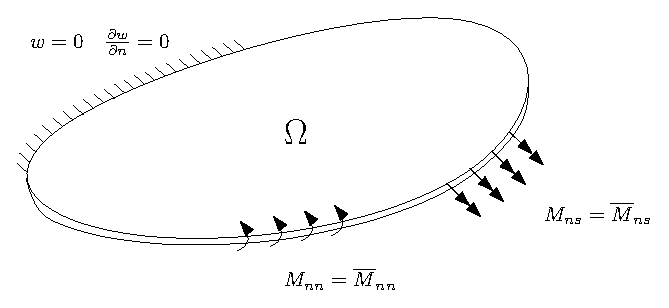
\includegraphics[width=0.7\textwidth]{Plate_Bcs.eps}
	\caption{Clamped plate with distributed torsional and flexural momenta at the border}
	\label{fig:mix_bcs}
\end{figure}

The port-Hamiltonian finite-dimensional system is rewritten equivalently by highlighting the known control terms, the Lagrange multipliers (reactions at the boundary) and the constraints, arising from the fact that, in the case of a non-moving boundary, $\bm{y}_{\lambda} = 0$
\begin{equation}
\begin{aligned}
\label{eq:PHdiscr_mixed}
\dot{\bm{\tilde{\alpha}}} &= J_d \bm{e}+ B P_{f} \bm{f}  + B P_{\lambda} \bm{\lambda}, \\
\bm{y}_{f} &= P_{f}^T B^T \bm{e}, \\
0 &= P_{\lambda}^T B^T \bm{e}. \\
\end{aligned}
\end{equation}

This port-Hamiltonian system is an algebraic-differential system which can be treated applying results detailed in \cite{vanderSchaft2013,beattie2017port}.



\section*{Conclusions and Perspectives}

In this paper the port-Hamiltonian formulation of the Mindlin plate was enriched by the equivalent tensorial formulation. The PFEM method proves again its versatility, since it stays valid and applicable even in more complicated examples like the one presented in this article. Its powerfulness is the capability of preserving the port-Hamiltonian structure. \\

Many open questions still remain, though. The discretized system can be easily implemented by a finite-element software, but the functional spaces in which the variables live need to be specified precisely. This is necessary to have a guarantee of convergence of the corresponding finite element method. 
Once the proper functional spaces are defined, different finite elements should be tested against several test-case scenarios. The selected basis functions should work no matter the boundary conditions. Once a valid choice has been made, it might be possible to interconnect the discretized plate model with a surrounding system, e.g. a multi-physics environment. A mathematical proof that this operation is possible should be studied as well. \\

Another important aspect is the implementation of suitable control laws. Passivity-based approaches and the energy shaping methods were already largely studied in the literature. It would be of great interest, especially for control engineers, to conceive a controller able to respect given performance specifications. The port-Hamiltonian formalism and its powerfulness in modeling complex systems could be linked to standard control methodologies, already well known in the industrial field.   

\section*{Acknowledgments}
This work is  supported by the project ANR-16-CE92-0028,
entitled {\em Interconnected Infinite-Dimensional systems for Heterogeneous
Media}, INFIDHEM, financed by the French National
Research Agency (ANR) and the Deutsche Forschungsgemeinschaft (DFG).
Further information is available at {\url{https://websites.isae-supaero.fr/infidhem/the-project}}.  \\
Moreover the author would like to thank Michel Sala\"un for the fruitful and insightful discussions
   
\bibliographystyle{unsrt}
\bibliography{biblio_Mindlin}
	
	
\end{document}
\endinput